% JOINT RANDOM VARIABLES
All things considered, Bayesian modeling rests on the marginal distribution \(\pi(\bm{x})\) of the unknown parameters in \cref{eq:Bayesian:PriorDensity}
and the conditional distribution \(\pi(\bm{y} \cond \bm{x})\) of the observational data in \cref{eq:Bayesian:DataModel}.
Consequentially the unknowns and the data are represented as jointly distributed random vectors
\begin{equation} \label{eq:Bayesian:JointDensity}
  (\bm{Y},\bm{X}) \sim \pi(\bm{y},\bm{x}) = \pi(\bm{y} \cond \bm{x}) \pi(\bm{x}).
\end{equation}
% BAYESIAN EXPERIMENT
This is a complete probability model of the Bayesian experiment.
The true parameters and the actual data are regarded as a realization \((\bm{Y},\bm{X}) = (\bm{y},\bm{x})\) of the joint random variables in \cref{eq:Bayesian:JointDensity}.
While the outcome of the data \(\bm{y}\) is observed, the true parameters \(\bm{x}\) remain unobserved.
\par % POSTERIOR DENSITY
Now one can synthesize the prior information and the observed data in order to estimate the unknowns.
In particular, one proceeds by conditioning on the realized data.
Given the likelihood function in \cref{eq:Bayesian:LikelihoodFunction} and the prior density in \cref{eq:Bayesian:PriorDensity},
the \emph{posterior density} follows from Bayes' law
\begin{gather}
  \pi(\bm{x} \cond \bm{y}) = \frac{\mathcal{L}(\bm{x}) \pi(\bm{x})}{\scale}, \label{eq:Bayesian:PosteriorDensity} \\
  \scale = \int\limits_{\mathds{R}^\dimParam} \mathcal{L}(\bm{x}) \, \pi(\bm{x}) \, \mathrm{d} \bm{x}. \label{eq:Bayesian:ModelEvidence}
\end{gather}
The normalizing constant \(\scale\) is usually called the \emph{model evidence} or \emph{marginal likelihood}.
It will be further examined in \cref{sec:Bayesian:ModelEvidence}.
In the same fashion as the prior represents the uncertainty about the unknowns before analyzing the data,
the posterior in \cref{eq:Bayesian:PosteriorDensity} summarizes the reduced uncertainty afterwards.
\par % ILLUSTRATION
In \cref{fig:Bayesian:BayesianInference} the functioning of Bayesian updating is illustrated for a single quantity of interest (QoI).
The prior is transited into the posterior density, which is paralleled by a reduction of the epistemic uncertainty and a higher degree of probability mass localization.
For the sake of clarity, both the prior and the posterior density in the sketch are Gaussian.
In most but the simplest cases, however, the posterior is a complex probability distribution that may exhibit strong non-normalities and a multiplicity of modes.
Multivariate posteriors often contain linear correlations and complex dependencies between the variables involved.
% FIGURE: BAYESIAN INFERENCE
\begin{figure}[htbp]
  \centering
  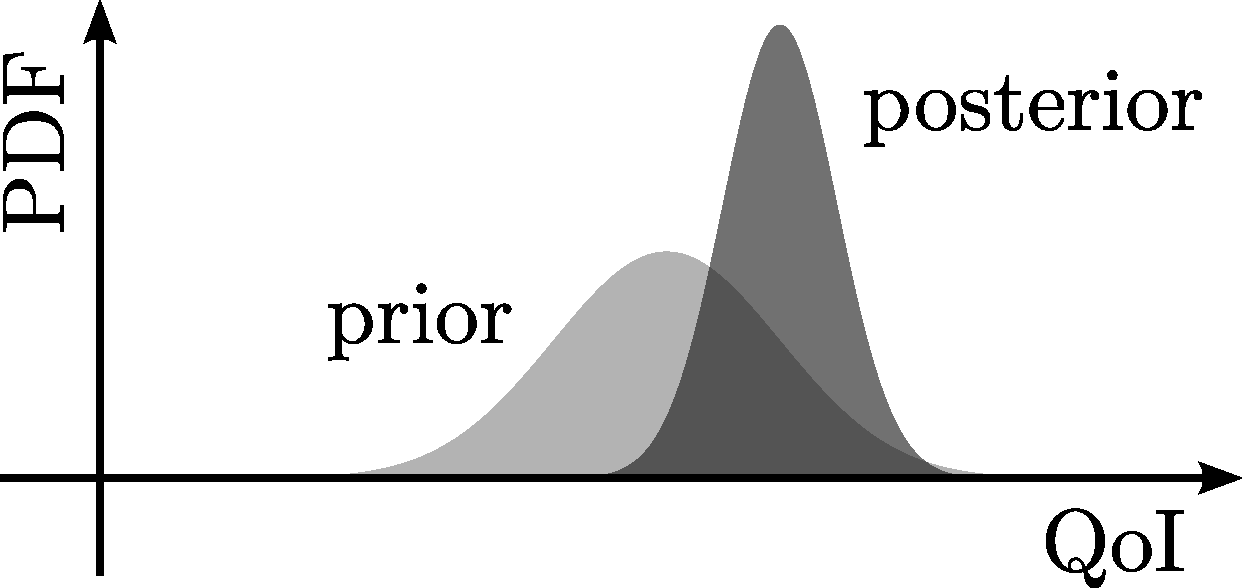
\includegraphics[width=6.66cm]{fig_Bayesian_BayesianInference}
  \caption[Bayesian inference]{Bayesian inference.}
  \label{fig:Bayesian:BayesianInference}
\end{figure}
\par % CONDITIONAL EXPECTATION/PROBABILITY
Now all information is contained in the posterior probability density function.
As opposed to the determination of the prior where the question was how to encode information into a probability density, the question here becomes how to decode it from the posterior.
A natural way is to evaluate conditional expectation values and regular probabilities given the data.
The expectation of a certain QoI \(h \colon \mathds{R}^\dimParam \rightarrow \mathds{R}\) under the posterior can be written as
\begin{equation} \label{eq:Bayesian:ConditionalExpectation}
  \mathds{E}[h(\bm{X}) \cond \bm{y}] = \int\limits_{\mathds{R}^\dimParam} h(\bm{x}) \, \pi(\bm{x} \cond \bm{y}) \, \mathrm{d} \bm{x}.
\end{equation}
Most relevant quantities follow thereby from considering appropriate QoIs.
For instance, with the indicator function \(h = I_B\) of a set \(B \in \mathcal{B}(\mathds{R}^\dimParam)\) one obtains the posterior probability of the event \(\bm{X} \in B\) as
\begin{equation} \label{eq:Bayesian:ConditionalProbability}
  \mathds{P}_{\bm{X} \cond \bm{Y}}(B \cond \bm{y}) = \int\limits_{B} \pi(\bm{x} \cond \bm{y}) \, \mathrm{d} \bm{x}.
\end{equation}
This completes the characterization of the posterior probability distribution.
Possibilities to further analyze and summarize the posterior are discussed below.

\subsection{Posterior summaries}
% FIRST MOMENTS
Very often one is interested in the first statistical moments of the posterior.
They serve as brief summaries of the possibly complex probability distribution.
The expected value and covariance matrix are given as
\begin{gather}
  \mathds{E}[\bm{X} \cond \bm{y}] = \int\limits_{\mathds{R}^\dimParam} \bm{x} \, \pi(\bm{x} \cond \bm{y}) \, \mathrm{d} \bm{x}, \label{eq:Bayesian:PosteriorMean} \\
  \mathrm{Cov}[\bm{X} \cond \bm{y}]
  = \int\limits_{\mathds{R}^\dimParam} (\bm{x} - \mathds{E}[\bm{X} \cond \bm{y}]) (\bm{x} - \mathds{E}[\bm{X} \cond \bm{y}])^\top 
  \pi(\bm{x} \cond \bm{y}) \, \mathrm{d} \bm{x}. \label{eq:Bayesian:PosteriorCovariance}
\end{gather}
The posterior mean in \cref{eq:Bayesian:PosteriorMean} is often taken as a point estimate of the unknown parameter vector,
whereas the covariance in \cref{eq:Bayesian:PosteriorCovariance} is regarded as a measure of the statistical uncertainty.
% MAP ESTIMATE
An alternative for point estimation is the \emph{maximum a posteriori} (MAP) estimate.
It maximizes the posterior density over the admissible parameter values.
Simply put, this is just the mode
\begin{equation} \label{eq:Bayesian:PosteriorMode}
  \hat{\bm{x}}_{\mathrm{MAP}} = \operatorname*{arg\,max}_{\bm{x} \in \mathds{R}^\dimParam} \pi(\bm{x} \cond \bm{y}).
\end{equation}
% CREDIBLE REGIONS
For interval estimation one usually specifies \emph{credible regions} that accumulate a certain high percentage of the total posterior mass.
The probability that such sets indeed contain the true parameter values is determined according to \cref{eq:Bayesian:ConditionalProbability}.
\par % BAYES ESTIMATOR
Bayesian point estimation can be more formally understood within a decision-theoretic framework \cite{Bayesian:Berger1985,Bayesian:Robert2007}.
A \emph{Bayes estimator} minimizes/maximizes the expected value of a certain loss/utility function under the posterior distribution.
The posterior mean in \cref{eq:Bayesian:PosteriorMean} is the Bayes estimator for a quadratic risk function.
Technically speaking, MAP estimation in \cref{eq:Bayesian:PosteriorMode} does not establish a proper Bayes estimator.
It can be understood as a limit of such, though.
\par % POSTERIOR MARGINALS
In the multivariate case, the joint posterior may contain dependencies between the components of \(\bm{x}\).
Although the presence or lack of such structures gives deep insight into the problem at hand, one may want to disregard them for the moment and focus on the posterior marginals.
For a specific parameter \(x_i\) with \(i \in \{1,\ldots,\dimParam\}\) one integrates the posterior over the remaining unknowns
\(\bm{x}_{\without i} = (x_1,\ldots,x_{i-1},x_{i+1},\ldots,x_\dimParam)^\top\) in order to obtain
\begin{equation} \label{eq:Bayesian:PosteriorMarginal}
  \pi(x_i \cond \bm{y}) = \int\limits_{\mathds{R}^{\dimParam-1}} \pi(\bm{x} \cond \bm{y}) \, \mathrm{d} \bm{x}_{\without i}.
\end{equation}
This summarizes the accumulated information on the parameter \(x_i\).
Since one-dimensional posterior marginals can be visualized nicely, they are often plotted as graphical summaries of the joint posterior.

\subsection{Predictive distributions}
% PRIOR PREDICTIVE DISTRIBUTION
In the same way as the prior \(\pi(\bm{x})\) informs about \(\bm{x}\), i.e.\ the distribution represents a subjective uncertainty rather than a sampling frequency,
our expectations on the data \(\bm{y}\) before seeing them are summarized by
\begin{equation} \label{eq:Bayesian:PriorPredictiveDistribution}
  \pi(\bm{y}) = \int\limits_{\mathds{R}^\dimParam} \pi(\bm{y} \cond \bm{x}) \, \pi(\bm{x}) \, \mathrm{d} \bm{x}.
\end{equation}
This is called the \emph{prior predictive density}.
The model evidence in \cref{eq:Bayesian:ModelEvidence} actually stems from evaluating the prior predictive density at the real data.
After analyzing the data \(\bm{y}\), one can similarly predict the future outcome \(\bm{y}^\prime\) in a replication of the experiment.
\par % FUTURE DATA
It is often assumed that the observed and the future data are conditionally independent.
This means that \(\pi(\bm{y},\bm{y}^\prime \cond \bm{x}) = \pi(\bm{y} \cond \bm{x}) \pi(\bm{y}^\prime \cond \bm{x})\).
The probabilistic data model in \cref{eq:Bayesian:DataModel} can then be adjusted to as yet unobserved data
\(\bm{Y}^\prime \sim \pi(\bm{y}^\prime \cond \bm{x})\), e.g.\ by resetting the covariates.
One could simply use \(\pi(\bm{y}^\prime \cond \hat{\bm{x}})\) for predicting the future data,
where \(\hat{\bm{x}}\) is some point estimate of the parameters that comes from an analysis of the old data.
% POSTERIOR PREDICTIVE DISTRIBUTION
This, however, ignores the statistical estimation uncertainty.
It is therefore advisable to average over the posterior so as to derive the \emph{posterior predictive density}
\begin{equation} \label{eq:Bayesian:PosteriorPredictiveDistribution}
  \pi(\bm{y}^\prime \cond \bm{y})
  = \int\limits_{\mathds{R}^\dimParam} \pi(\bm{y}^\prime \cond \bm{x},\bm{y}) \, \pi(\bm{x} \cond \bm{y}) \, \mathrm{d} \bm{x}
  = \int\limits_{\mathds{R}^\dimParam} \pi(\bm{y}^\prime \cond \bm{x}) \, \pi(\bm{x} \cond \bm{y}) \, \mathrm{d} \bm{x}.
\end{equation}
The second equality is a direct consequence of the conditional independence \(\pi(\bm{y}^\prime \cond \bm{x},\bm{y}) = \pi(\bm{y}^\prime \cond \bm{x})\).
Similar to the unconditional data predictions in \cref{eq:Bayesian:PriorPredictiveDistribution},
the distribution in \cref{eq:Bayesian:PosteriorPredictiveDistribution} predicts new data given the already observed ones.

\subsection{Information gain}
% INFORMATION THEORY
It is interesting to look at the Bayesian update from an information-theoretic point of view \cite{Bayesian:Lindley1956,Bayesian:Lindley1972}.
This is of paramount importance for Bayesian optimal design \cite{Bayesian:Bernardo1979:a,Bayesian:Chaloner1995}
and the definition of least-informative reference priors \cite{Bayesian:Bernardo1979:b,Bayesian:Berger2009}.
A more specific perspective on the pervasive concepts of ``information'' and ``uncertainty''
and their embodiment in probability distributions is entailed hereby \cite{Statistics:Cover2006,Statistics:Gray2011}.
\par % SHANNON ENTROPY
Intuitively one may think of information as the complement of uncertainty.
More formally it can be interpreted as the reduction of uncertainty \(-\log \pi(\bm{x})\) that results
from receiving the outcome \(\bm{X} = \bm{x}\) of a random variable \(\bm{X} \sim \pi(\bm{x})\).
Note that this does not describe a Bayesian learning procedure.
The \emph{Shannon entropy} quantifies the potential information gain or average surprisal \(\mathds{E}[-\log \pi(\bm{X})]\)
of this communication process \cite{Statistics:Shannon1948:a,Statistics:Shannon1948:b}.
This way it rigorously measures the degree of unpredictability or uncertainty that is inherent in a whole probability distribution.
% INFORMATION ENTROPY
The entropy of the continuous prior density \(\pi(\bm{x})\) is defined as
\begin{equation} \label{eq:Bayesian:InformationEntropy}
  H_{\mathrm{S}}(\pi(\cdot)) = - \int\limits_{\mathds{R}^\dimParam} \log(\pi(\bm{x})) \, \pi(\bm{x}) \, \mathrm{d} \bm{x}.
\end{equation}
Likewise one can define the information entropy \(H_{\mathrm{S}}(\pi(\cdot \cond \bm{y}))\) of the posterior density \(\pi(\bm{x} \cond \bm{y})\).
Notice that the differential entropy in \cref{eq:Bayesian:InformationEntropy} may become negative and is not invariant under a change of variables.
Actually, these undesirable properties have arisen due to the transfer of the original definition from discrete to continuous random variables.
\par % RELATIVE ENTROPY
A relative entropy concept that works equally well in the discrete and the continuous case is the
\emph{Kullback--Leibler} (KL) \emph{divergence} \cite{Statistics:Kullback1951,Statistics:Kullback1968}.
It measures the additional entropy that is introduced when using an approximate or distorted distribution in place of the true reference one.
While the actual events follow the reference, they are incorrectly expected according to the approximation.
The additional uncertainty of predicting the posterior \(\pi(\bm{x} \cond \bm{y})\) as the reference with the prior \(\pi(\bm{x})\) as the approximation can be defined as
\begin{equation} \label{eq:Bayesian:RelativeEntropy}
  D_{\mathrm{KL}}(\pi(\cdot \cond \bm{y}) \| \pi(\cdot))
  = \int\limits_{\mathds{R}^{\dimParam}} \log \left( \frac{\pi(\bm{x} \cond \bm{y})}{\pi(\bm{x})} \right) \pi(\bm{x} \cond \bm{y}) \, \mathrm{d} \bm{x}
  = - \int\limits_{\mathds{R}^{\dimParam}} \log(\pi(\bm{x})) \, \pi(\bm{x} \cond \bm{y}) \, \mathrm{d} \bm{x} - H_{\mathrm{S}}(\pi(\cdot \cond \bm{y})).
\end{equation}
The cross-entropy \(H_{\mathrm{C}}(\pi(\cdot \cond \bm{y}),\pi(\cdot)) = - \int_{\mathds{R}^{\dimParam}} \log(\pi(\bm{x})) \, \pi(\bm{x} \cond \bm{y}) \, \mathrm{d} \bm{x}\)
measures the total uncertainty of using the prior instead of the true posterior.
Hence, the relative entropy in \cref{eq:Bayesian:RelativeEntropy} is the additional uncertainty
\(D_{\mathrm{KL}}(\pi(\cdot \cond \bm{y}) \| \pi(\cdot)) = H_{\mathrm{C}}(\pi(\cdot \cond \bm{y}),\pi(\cdot)) - H_{\mathrm{S}}(\pi(\cdot \cond \bm{y}))\).
It is a non-negative and transformation-invariant measure of the difference between two probability distributions in terms of their entropy contents.
Moreover, the divergence is asymmetric by construction and attains zero if and only if \(\pi(\bm{x} \cond \bm{y}) = \pi(\bm{x})\).
\par % BAYESIAN UPDATE
Following these remarks, one can interpret the KL divergence \(D_{\mathrm{KL}}(\pi(\cdot \cond \bm{y}) \| \pi(\cdot))\)
as a measure of the uncertainty reduction that comes along with the passage from the prior to the posterior.
This may be seen as the amount of information brought by the data in turn.
It is worth mentioning here that this measure of the information gain is never negative, no matter of how the distributions look like,
and regardless of whether the divergence from the prior to the posterior or from the posterior to the prior is considered.